\documentclass{beamer}
\usetheme{metropolis}
\usepackage[utf8]{inputenc}
\usepackage[T1]{fontenc}
\usepackage{listings}
\usepackage{xcolor}
\usepackage{tikz}
\usetikzlibrary{arrows.meta, positioning, shapes.geometric}

\lstdefinestyle{cpp}{
  language=C++,
  basicstyle=\ttfamily\tiny,
  keywordstyle=\color{blue!70!black}\bfseries,
  commentstyle=\color{gray}\itshape,
  stringstyle=\color{orange!80!black},
  breaklines=true,
  breakatwhitespace=false,
  columns=fullflexible,
  keepspaces=true,
}
\lstset{style=cpp}

\title{SolTrace Result API Redesign}
\subtitle{Reducing data movement and enabling flexible result types}
\date{\today}

\begin{document}

\maketitle

% ─────────────────────────────────────────────────────────────────────────────
\section{Motivation}
% ─────────────────────────────────────────────────────────────────────────────

\begin{frame}{Problem: One rigid result type}
\textbf{Before}: \lstinline|report_simulation| always builds a full ray history.
\begin{itemize}
  \item Every hit $\rightarrow$ heap-allocated \lstinline|shared_ptr<InteractionRecord>|
  \item All ray paths grouped into \lstinline|RayRecord| objects
  \item Per-element \lstinline|element_view| map always constructed
  \item GPU runner downloads the full compacted hit buffer unconditionally
\end{itemize}
\vspace{0.5em}
\textbf{Many use cases only need a subset of this data}, e.g.:
\begin{itemize}
  \item Flux per element (no per-ray records needed)
  \item Hits on a specific subset of elements
  \item Raw hit buffer for custom post-processing
\end{itemize}
\end{frame}

\begin{frame}[fragile]{Old API}
\begin{lstlisting}
// SimulationRunner
virtual RunnerStatus setup_simulation(
    const SimulationData *data) = 0;

virtual RunnerStatus report_simulation(
    SimulationResult *result,   // single concrete type
    int level_spec) = 0;        // unused parameter

// Caller
SimulationResult result;
runner.setup_simulation(&data);
runner.run_simulation();
runner.report_simulation(&result, 0);
\end{lstlisting}
\begin{alertblock}{Issues}
\begin{itemize}
  \item No way to request a lighter-weight result
  \item Runner cannot configure GPU buffers for the desired output
  \item \lstinline|level_spec| was unused but required
\end{itemize}
\end{alertblock}
\end{frame}

% ─────────────────────────────────────────────────────────────────────────────
\section{Result Type Hierarchy}
% ─────────────────────────────────────────────────────────────────────────────

\begin{frame}[fragile]{Step 1: Abstract base + \texttt{ResultType} enum}
\begin{lstlisting}
enum class ResultType { RAY_HISTORY, ELEMENT_STATS, RAW_HITS };

class SimulationResult {  // abstract base
public:
    virtual ~SimulationResult() = default;
    virtual ResultType get_result_type() const = 0;
    // Sun metadata common to all result types
    void set_sun_ray_count(uint_fast64_t n);
    void set_sun_dimensions(double w, double h);
    void set_sun_A_box(double A);
protected:
    SimulationResult() = default;
};

class RayHistoryResult : public SimulationResult {  // concrete
public:
    ResultType get_result_type() const override
        { return ResultType::RAY_HISTORY; }
    // RayRecord, InteractionRecord, element_view ...
};
\end{lstlisting}
\end{frame}

\begin{frame}{Result type hierarchy}
\begin{center}
\resizebox{\textwidth}{!}{%
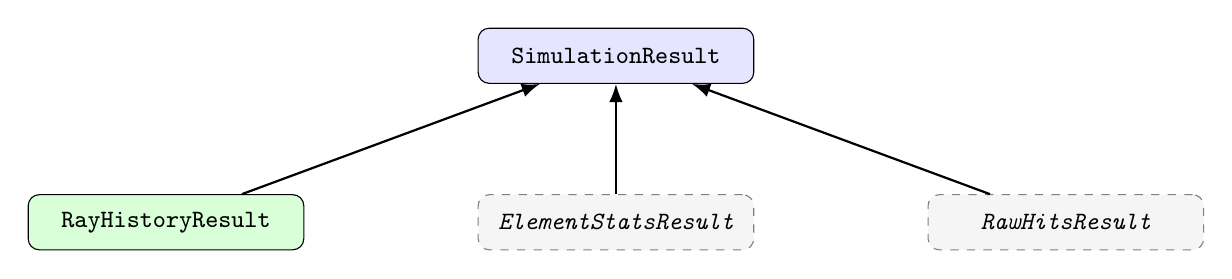
\begin{tikzpicture}[
    node distance=1.4cm and 2.2cm,
    abstract/.style={rectangle, draw, fill=blue!10,
                     rounded corners, minimum width=3.5cm, minimum height=0.7cm,
                     font=\ttfamily\small},
    concrete/.style={rectangle, draw, fill=green!15,
                     rounded corners, minimum width=3.5cm, minimum height=0.7cm,
                     font=\ttfamily\small},
    future/.style={rectangle, draw=gray, dashed, fill=gray!8,
                   rounded corners, minimum width=3.5cm, minimum height=0.7cm,
                   font=\ttfamily\small\itshape},
    arr/.style={-{Latex}, thick},
]
  \node[abstract] (base) {SimulationResult};
  \node[concrete, below left=of base]  (rh)  {RayHistoryResult};
  \node[future,   below=of base]       (es)  {ElementStatsResult};
  \node[future,   below right=of base] (raw) {RawHitsResult};

  \draw[arr] (rh)  -- (base);
  \draw[arr] (es)  -- (base);
  \draw[arr] (raw) -- (base);
\end{tikzpicture}%
}
\end{center}
\vspace{0.4em}
\begin{itemize}
  \item \texttt{SimulationResult} carries sun metadata — no cast needed to set it
  \item \texttt{RayHistoryResult} holds full per-ray interaction history
  \item Dashed types are future result shapes, not yet implemented
\end{itemize}
\end{frame}

% ─────────────────────────────────────────────────────────────────────────────
\section{Result Spec Hierarchy}
% ─────────────────────────────────────────────────────────────────────────────

\begin{frame}[fragile]{Step 2: \texttt{ResultSpec} — configuration + factory}
\begin{lstlisting}
struct ResultSpec {
    virtual ResultType get_type() const = 0;
    // Factory: creates the matching empty result container
    virtual std::unique_ptr<SimulationResult> create_result() const = 0;
    // Configuration queries — default = no filter (record everything)
    virtual std::optional<std::set<element_id>>
        get_element_filter() const { return std::nullopt; }
    virtual std::optional<std::set<RayEvent>>
        get_event_filter() const { return std::nullopt; }
};

struct RayHistorySpec : ResultSpec {
    std::optional<std::set<element_id>> element_filter;
    std::optional<std::set<RayEvent>>   event_filter;

    ResultType get_type() const override
        { return ResultType::RAY_HISTORY; }
    std::unique_ptr<SimulationResult> create_result() const override
        { return std::make_unique<RayHistoryResult>(); }
    // overrides get_element_filter() and get_event_filter()
};
\end{lstlisting}
\end{frame}

\begin{frame}{Why separate spec from result?}
\begin{columns}[T]
\column{0.48\textwidth}
\textbf{ResultSpec} (input / configuration)
\begin{itemize}
  \item Passed to \lstinline|setup_simulation()|
  \item Runner reads it to configure GPU buffers, filters before any ray is traced
  \item Owns the factory method
  \item Short-lived; caller keeps it
\end{itemize}
\column{0.48\textwidth}
\textbf{SimulationResult} (output / data)
\begin{itemize}
  \item Created by \lstinline|create_result()|
  \item Passed to \lstinline|report_simulation()|
  \item Runner populates it after tracing
  \item Long-lived; caller owns and queries it
\end{itemize}
\end{columns}
\vspace{1em}
\begin{block}{Key property}
Type mismatch between setup and report is eliminated: the spec that configures the runner is the same object that creates the result container.
\end{block}
\end{frame}

% ─────────────────────────────────────────────────────────────────────────────
\section{Updated Runner Interface}
% ─────────────────────────────────────────────────────────────────────────────

\begin{frame}[fragile]{Updated \texttt{SimulationRunner} interface}
\begin{lstlisting}
class SimulationRunner {
public:
    // Spec default = RayHistorySpec{}: existing call sites unchanged
    virtual RunnerStatus setup_simulation(
        const SimulationData *data,
        const ResultSpec     &spec = RayHistorySpec{}) = 0;

    virtual RunnerStatus run_simulation() = 0;

    // Runner-side factory based on stored ResultType
    virtual std::unique_ptr<SimulationResult> create_result() = 0;

    // Accepts abstract base; level_spec default preserves compat
    virtual RunnerStatus report_simulation(
        SimulationResult *result, int level_spec = 0) = 0;
};
\end{lstlisting}
\begin{itemize}
  \item \lstinline|report_simulation| accepts \lstinline|SimulationResult*|;
        runners \lstinline|dynamic_cast| internally for type-specific work
\end{itemize}
\end{frame}

\begin{frame}[fragile]{New call pattern}
\begin{lstlisting}
// --- Filter to two specific elements ---
RayHistorySpec spec;
spec.element_filter = { receiver_id, target_id };

runner.setup_simulation(&data, spec);  // runner configures buffers/filters
runner.run_simulation();

// Two equivalent ways to get the result container:
auto result = spec.create_result();    // spec still in scope
auto result = runner.create_result();  // runner uses stored ResultType

runner.report_simulation(result.get());

// --- Existing code: unchanged ---
runner.setup_simulation(&data);        // default RayHistorySpec, no filter
runner.run_simulation();
SimulationResult *r = ...;
runner.report_simulation(r, 0);        // legacy two-arg form compiles
\end{lstlisting}
\end{frame}

% ─────────────────────────────────────────────────────────────────────────────
\section{Runner Implementation}
% ─────────────────────────────────────────────────────────────────────────────

\begin{frame}[fragile,shrink=5]{Inside a runner: setup \& report}
\begin{lstlisting}
// setup: extract configuration from the spec
RunnerStatus NativeRunner::setup_simulation(
    const SimulationData *data, const ResultSpec &spec)
{
    m_result_type = spec.get_type();
    // future: m_element_filter = spec.get_element_filter();
    // ... existing GPU/CPU setup ...
}

// create_result: runner-side factory
std::unique_ptr<SimulationResult> NativeRunner::create_result()
{
    switch (m_result_type) {
        case ResultType::RAY_HISTORY:
            return make_unique<RayHistoryResult>();
        default: return nullptr;
    }
}

// report_simulation: safe downcast, ERROR on type mismatch
RunnerStatus NativeRunner::report_simulation(
    SimulationResult *result, int)
{
    auto *r = dynamic_cast<RayHistoryResult *>(result);
    if (!r) return RunnerStatus::ERROR;
    // ... populate r ...
}
\end{lstlisting}
\end{frame}

% ─────────────────────────────────────────────────────────────────────────────
\section{Summary}
% ─────────────────────────────────────────────────────────────────────────────

\begin{frame}{Summary of changes}
\resizebox{\textwidth}{!}{%
\begin{tabular}{lll}
\hline
& \textbf{Before} & \textbf{After} \\
\hline
Result base & (none) & \texttt{SimulationResult} \\
Concrete result & \texttt{SimulationResult} & \texttt{RayHistoryResult} \\
Runner config & \texttt{ResultType} enum & \texttt{ResultSpec} hierarchy \\
Factory & (none) & \texttt{spec.create\_result()} / \texttt{runner.create\_result()} \\
\texttt{setup\_simulation} & \texttt{(SimulationData*)} & \texttt{(SimulationData*, ResultSpec\&)} \\
\texttt{report\_simulation} & \texttt{(SimulationResult*, int)} & \texttt{(SimulationResult*, int=0)} \\
Type mismatch & Runtime only & Eliminated at boundary \\
Backward compat & --- & All call sites unchanged \\
\hline
\end{tabular}%
}
\end{frame}

\begin{frame}{Adding a new result type}
Adding \texttt{ElementStatsResult} (future work) requires:
\begin{enumerate}
  \item New \lstinline|ElementStatsResult : SimulationResult| class with per-element fields
  \item New \lstinline|ElementStatsSpec : ResultSpec| with its configuration parameters and \lstinline|create_result()| returning \lstinline|make_unique<ElementStatsResult>()|
  \item Add \lstinline|case ResultType::ELEMENT_STATS| to each runner's \lstinline|create_result()| and \lstinline|report_simulation()|
\end{enumerate}
\vspace{0.5em}
No changes required to:
\begin{itemize}
  \item The \texttt{SimulationRunner} interface
  \item Existing spec or result classes
  \item Any existing call sites
\end{itemize}
\end{frame}

\end{document}
